\documentclass[UTF8]{ctexart}
\usepackage{shumo}%可以点开查看宏包和定义内容,同时可以自行另外加宏包和定义
\geometry{left=2.50cm,right=2.5cm,top=2.50cm,bottom=2.5cm}%页面布局集训标准,可自行适当修改
%====================================================
%设置附录代码的格式,可以自行修改
\lstset{
	breaklines=true,% 允许自动断行
	% breakatwhitespace=true,% 使用此命令仅允许在空格处自动断行
	showstringspaces=false,% 不显示字符串中的空格
	basicstyle=\small\ttfamily,% 设置代码基本样式
	flexiblecolumns=true,% 改善字母间距
	keywordstyle=\color{blue},% 设置关键词样式
	stringstyle=\color[rgb]{0.75,0,0.75},% 设置字符串样式
	commentstyle=\songti\color[rgb]{0,0.5,0},% 设置注释样式
	tabsize=4,% 设置制表符缩进
}
%====================================================
\title{\textbf{基于启发式二分搜索的城市轨道交通列车时刻表优化研究}}% 请勿修改
\date{}%请勿添加自己的信息
\author{}%请勿添加自己的信息
%下面时正文
\begin{document}
\setcounter{page}{1}%从正文开始计算页码	
\maketitle
\vspace{-0.95cm}
\thispagestyle{fancy}   
\fancyhf{} %清除原本页眉页脚形式
\renewcommand{\headrulewidth}{0pt} %页眉线宽,设为0可以去页眉线
%=================================================
%=================================================
%=================================================
%=================================================
%=================================================
%=================================================
%下面开始出现各位需要修改的部分。
	\renewcommand{\abstractname}{\sihao 摘\quad 要} %更改摘要二字的样式
\begin{abstract}\xiaosihao
	\vspace{0.1cm}
	城市轨道交通是大城市公共交通的重要组成部分,随着城市规模的不断扩大和人口的增加,轨道交通的客流量也在不断增加。因此,如何优化城市轨道交通列车时刻表,提高列车的运营效率和客运能力,已成为一个亟待解决的问题。\par 
	针对问题一,本文先通过查阅文献和关键指标转化将问题简化,主要采用C++代码实现,首先运用贪心算法达到企业运营成本最小化。后两次运用二分搜索法,第一次枚举小交路列车数量确定其数量区间,第二次枚举小交路列车运行长度,确定其运行列数。最后建立多约束受限,多主体协同下两个目标函数的多目标规划模型,数值计算优化调度列车开行方案。\par 
	针对问题二,基于模型一所建立模型由层次分析法得到各个站点的权值,来确定乘客人数高谷站点,及时满足乘客的需求使服务水平最大化。依据列车交替开行的运营模式,考虑时间安全间隔,得到列车发行的时刻表,制定等间隔的平行运行图。\par 
	针对问题三,要改变列车类型及编组数量,增加列车定员,提升列车最大载客量,从而减少列车数量,降低乘客候车时间,实现企业运营成本最小化和服务水平最大化目标,使得模型再次优化。
	最后,对模型进行了优缺点分析,对模型进行改进策略并进行推广。\par 
	
	
	
	%这里填写你自己的关键词
	
	\textbf{关键词}:\quad 列车时刻优化表,贪心算法,二分搜索法,多目标规划,层次分析法
\end{abstract}

\newpage

\pagestyle{plain}
%标准 LaTeX 提供下列四种页版式,可用 \pagestyle{页版式} 命令来设置页面版式:
%empty(没有页眉和页脚),plain(本次用的,无页眉,页脚为居中页码),headings(页眉为章节标题,无页脚),myheadings(页眉内容可自定义,无页脚)


\section{问题背景}
\subsection{问题背景}
城市轨道交通列车时刻表优化问题是一个十分重要的问题,涉及到城市公共交通的服务质量、运营效率和安全等多个方面。需要运用多种方法和技术进行研究和优化,以提高城市轨道交通的服务水平,更好地服务城市居民。城市轨道交通列车时刻表的优化涉及多个方面,包括列车的发车时间、停站时间、运行速度、列车班次等等。优化列车时刻表需要考虑到列车之间的间隔时间、站点之间的距离、客流峰值时段等因素,同时还需要充分考虑列车运营安全和客运质量等方面的要求。\par
因此,城市轨道交通列车时刻表优化问题是一个复杂的问题,需要运用运筹学、数学模型等方法,结合实际情况进行研究和优化,以提高城市轨道交通的运营效率和服务质量。此外,随着科技的不断发展,城市轨道交通列车时刻表的优化也涉及到智能化技术的应用。例如,可以利用数据挖掘、人工智能等技术对客流数据进行分析,预测客流量峰值时段和客流集中的站点,从而更加科学地制定列车时刻表。\par
在优化列车时刻表的过程中,还需要考虑到列车运行的稳定性和安全性。例如,在考虑列车发车时间和停站时间时,需要充分考虑列车之间的间隔时间,以确保列车之间的安全距离,并避免发生事故。此外,还需要充分考虑列车维修、清洁等因素,以保证列车的运行安全和乘客的舒适性。\par
要制定一个列车开行方案如图,在考虑列车发车时间和停站时间时,充分考虑列车之间的间隔时间,确保列车之间的安全距离,避免发生事故。\par
实际运营中,在铺画列车运行图之前,首先得先确定列车开行方案,列车开行方案包括\textbf{列车编组方案、列车停站方案和列车交路计划}三部分。\par
列车编组方案规定了列车的车型和编组数量(即列车的节数),在本问题中采用统一的车型和编组数量。\par
\subsection{问题重述}
根据题目背景及所给附件,我们需要解决以下问题:\par
1.由题目可知题目中统一了车型和编组方案,要求再满足客流需求的条件下,制定合理的列车开行方案,包括分别确定大交路、小交路区间列车的运行区间以及开行数量,同时要达到企业运营成本最小化和服务水平最大化且尽量满足客流需求。\par
2.基于问题一制定的列车开行方案,加入时间要素,按满足客流需求及车辆行驶安全间隔下,再次优化模型,使问题考虑更趋向于现实,达到企业运营成本最小化和服务水平最大化的要求目标来制定等间隔的平行运行图。\par
3.对于降低企业运营成本和提高服务水平,基于已分析结果,创新性做出优化的列车开行方案,并对客流和车站数据分别提供相应的数据量化对比,展现出新列车开行方案的有效性,科学性。\par

\section{问题分析}
\subsection{问题一的分析}
\subsubsection{企业运营成本最小化}
通过分析,由题目已知信息可知,企业运营成本分为固定成本和变动成本,其中固定成本为车辆调度下每日所需调度固定成本,由于题目中限定了列车编组方案,确定了列车的车型和编组数量,在本问题中采用统一的车型和编组数量。因此假定选择车辆调度数量为固定成本的关键指标。变动成本则为车辆运行状态下,所需维持车辆正常运转消耗的油费,电费。因此假定车辆所运行的总路线为变动成本的关键指标。\par
\subsubsection{服务水平最大化}
通过分析,由题目已知信息可知,服务水平为乘客在车时间和乘客等待时间,其中乘客在车时间为乘客从上车到下车所经过的时间,包括列车区间运行时间和停站时间两部分组成,其中列车在车站的停站时间正比于在该站上,下车的乘客数量,但由附件 5 其他数据可知,乘客平均上下车时间仅为 0.04s,列车定员为 1860 人,平均停站时间为 74.4s,其中最小/大停站时间范围为[20-120]s,因此车辆人数承载最大化时乘客在车时间最佳。同时乘客等待时间为乘客在站台候车的等待时间,即为乘客到达站点后,第一个经过此站点的车辆,所需要的时间间隔。因此此时间间隔最小化时乘客等待时间最短,整体服务水平最大化。\par
\subsubsection{制定列车开行方案}
我们首先制定列车开行方案,即确定大交路和小交路的开行数量。通过合理安排大交路和小交路的开行数量,更好地满足不同区间的乘客需求, 提高运营效率。这意味着我们需要在不同车站之间合理分配列车开行数量, 以便在任何时段都能提供足够的运力。\par
本文根据所给的客流量即运营情况制定列车开行方案,反映企业运营成本和服务水平指标,建立多约束受限,多主体协同下乘客利益和企业利益两个目标函数的多目标规划数学模型。基于多目标规划分析法,进行数值计算,优化调度模型。\par
\subsection{问题二的分析}
基于问题一制定的能在满足乘客需求的前提下,实现运营成本的最小化和服务水平的最大化的列车开行方案,加入时间维度分析。考虑列车区间运行时间和停站时间的影响,并增加了安全间隔的限定,以此制定等间隔的平行运行图,其能够展示每趟列车在每个车站的到达和出发时间。\par 
相当于计算每趟列车的出发和到达时间时,在列车时序安排上,相同时空下,后车的进站时间不能等于前车的进站时间,并且必须两者相差时间大于安全间隔。保持较短的乘客等待时间,同时合理的出发间隔和停站时间可以确保乘客在车时间较短。提供便捷、准时的服务,让乘客能够在合理的时间内到达目的地。同时降低运营成本,提高运营效率。\par 
增加条件后,使模型更加真实合理,得到结果更符合实际。\par 
\subsection{问题三的分析}
基于题目所给出大小交列车模式的要求下,问题一与问题二已得出在规定的列车编组方案下使企业运营成本最小化和服务水平最大化的最优运行方案,若再次改善优化模型,则从列车开行方案中另一要素 列车编组方案出发,实现对目标再次优化。\par
\section{假设与符号说明}
\subsection{基本假设}
为了便于问题研究,对当前题目中某些条件进行合理的假设:\par
1.假设列车停站时间仅由乘客数量和其相关正比系数决定;\par
2.假设列车运行的速度恒定且相等;\par
3.假设题目所要求列车编组方案中规定的列车的车型和编组数量合理符合实际;\par
4.假设所设定安全间隔下列车理想状态下运行不发生冲突;\par
5.假设站点乘客人数变化为乘客上下车的人数;\par
6.乘客方面:不考虑由乘客性别,年龄等因素造成上下车的动作快慢;\par
7.驾驶员方面:不考虑由驾驶员的驾驶技术和反应速度等因素;\par
8.列车方面:不考虑列车突发事故,影响正常运行;\par
\subsection{符号说明}
\begin{table}[htbp]
	\centering 
	\begin{tabular}{lcr}
		\toprule
		变量名 & 符号说明  \\
		\midrule
		$s\left[ i \right] $ &各个站点的坐标(到车站1的距离) \\
		$t\left[ i \right] $ & 到达各个站点的时刻(假定从车站1出发是0时刻)  \\
		$big\_nt$ & 开行方案中大交路的数量  \\
		$small\_nt$ & 开行方案中小交路的每一站点最小列车数量 \\
		$big\_axx$& 大交路列车载客量  \\
		$big\_apacity$& 列车最大载客量  \\
		$nums\left[ i \right] $& 断面客流量 \\
		$st\left[ i \right] $& 大交路列车安排后,每一站点小交路列车所需承载的断面客流量 \\
		$s\_not$& 标记车站是否为具有折返能力的车站  \\
		$true$& 不具有折返能力的车站  \\
		$false$& 具有折返能力的车站  \\
		$must\_nt$& 列车数目为单位的总客流量  \\
		$vis\left[ i \right] $& check函数中站点临时已承载以列车数量为单位客流量  \\
		$cur$& check 函数中临时承载客流量  \\
		$tt\left[ i \right] $& 每一站点由乘客上下车所需的时间  \\
		$p\left[ i \right] $& 每一站点所占的权重  \\
		$nm\left[ i \right] $& 单位时间下单向路程下各个站点到此站点的客流量  \\
		$nm\left[ i \right] \left[ j \right] $& 单位时间下起始点为i,终止点为j的乘客人数  \\
		$sum\_axx$& 总客流量  \\
		$Rk$& 站点权值排名(以降序排列) \\
		\bottomrule
	\end{tabular}
\end{table}
\section{模型准备}
\subsection{列车运行区间数据预处理}
为方便对后续问题进行计算,首先对附件 2 中的临近车站的区间运行时间/车间距,进行预处理。得出任意两处车站间的区间运行时间/车间距, 进而得到任意两站点的路径矩阵,称为起-末矩阵。从而依据每一站点到车站1的位置为横坐标值建立坐标系,并标明车站属性(是否可作为交路起点/终点)。\par
具体过程分为如下步骤:\par
1.首先读入附件2中每一相邻车站的区间运行时间/车间距;\par
2.设置与车站数量相等大小的一维数组,依据一维前缀和算法,不断累加相邻车站的区间运行时间/车间距,从而得到任意车站到车站1的区间运行时间/车间距,即该一维数组为前缀和数组;\par
3.开辟一个(大小为[车站数量$\times$车站数量])二维数组,经历两重循环将枚举站点为起始站点和终止站点,并用新开辟的二维数组记录对应终止站点,起始站点前缀和数组的差值,即该二维数组为任意不同站点间区间运行时间/车间距,得到结果见附录1。\par
\section{模型建立}
\subsection{问题一}
由题目信息可知,在大小交路方案中(大小交路列车开行列数通常为1:n或n:1两种模式),查阅文献中大交路的概念可知,大交路的范围为全程。由贪心算法的思想,要使目标大小交路列车运行的路线总长度最短, 则先将大交路列车运行范围覆盖到全程,其中列数即满足全程中最少客流量所需的列车数目,后来由二分法调整短交路的运行区间和运行列数,因小交路列车的特性(小交路只有在具有折返能力的车站,才能作为交路的起点或终点),写check函数如图1。\par
\begin{figure}[h]
	\centering
	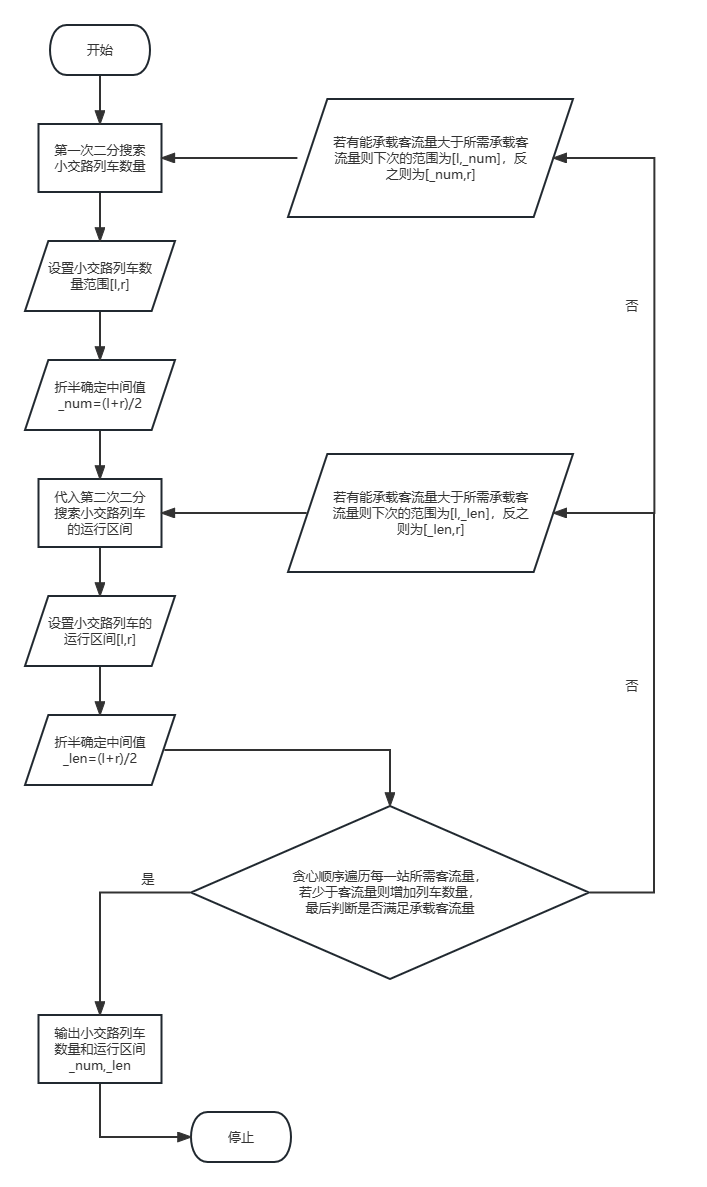
\includegraphics[scale=0.41]{模型一设计.png}
	\caption{模型一设计}
\end{figure}
设$s\left[ i \right]$为各个站点的坐标(到车站1的距离),如$s\left[ 1 \right] $为$0km$,$s\left[ 2 \right] $为$1.38km$。\par
设$t\left[ i \right]$为到达各个站点的时刻(假定从车站1出发是为0时刻),如$t\left[ 1 \right] $为$0h$,$t\left[ 2 \right] $为$120s$。\par
设$cnt_{big}$为开行方案中大交路的数量,$cnt_{small}$为开行方案中小交路的每一站点最小列车数量。\par
设$maxx_{big}$为大交路列车载客量,$capacity_{big}$为列车最大载客量。设$nums\left[ i \right]$为断面客流量,设$nums\left[ 1 \right]$为车站1—>车站2断面客流量,$nums\left[ 2 \right]$为车站 2—>车站3断面客流量…,$nums\left[ 30 \right]$为车站29—>车站30的断面客流量。\par
设$st\left[ i \right]$为大交路列车安排后,每一站点小交路列车所需承载的断面客流量,$st\left[ 1 \right]$为车站1—>车站2,车站2—>车站3…,车站29—>车站30的更新后的断面客流量。\par
设$is\_not$为标记车站是否为具有折返能力的车站,true为不具有折返能力的车站,false为具有折返能力的车站。\par
设$must\_cnt$为列车数目为单位的总客流量。\par
设$vis\left[ i \right]$为check函数中站点临时已承载以列车数量为单位客流量设$cur$为check函数中临时承载客流量大交路列车数量的安排:\par
由贪心算法的思想并结合现实实际可知,大交路的范围为列车行驶全站,因此若多增加大交路列车,会导致大小交路列车运行的总路线增加, 同时列车的满载率下降,会使企业运营成本中固定成本和变动成本增加, 因此优先安排大交路的数量,由于大交路全程覆盖的特点,可以安排大交路数量为全程中客流量最少的站点所需的列车个数,其中所需的列车个数则为客流量/列车载客量。\par
小交路列车数量的安排:\par
大交路列车数量安排后,则每一站点所负载的客流量更新为原站点载客量减去大交路列车的载客量,在这里即为减去大交路列车数量$\times $列车载客量,后由两次二分法,具体得出小交路列车的数量,区间范围最优安排。\par
第一次二分,枚举小交路列车的数量。由小交路运行长度最短为一站,同时一个站点所需最少列车数量为客流量/列车载客量,则小交路在站点最大列车数量为最大客流量/列车载客量,因此确定小交路列车的数量区间为[1,30*小交路最大列车数量];\par
第二次二分,枚举小交路列车的运行长度。由第一次二分可确定出小交路列车的数量,在此基础上,选择小交路列车的运行长度。由题目中小交路列车中只有具有折返能力的车站才能作为交路的起点或终点的特性写check 判断函数,最终确定小交路列车的安排方案。\par
根据问题要求,目标函数为企业运营成本最小化和服务水平最大化,可以总结为:\par
$$
\min \sum_{i=1}^n{C_i}+\alpha \sum_{j=1}^m{S_j}
$$
$$
s.t.\left\{ \begin{array}{c}
	\sum_{i=1}^n{X_{i,j}}+\sum_{k=1}^p{Y_{k,j}}=D_j,\forall j\\
	\sum_{i=1}^n{X_{i,j}}T_{i,j}+\sum_{k=1}^p{Y_{k,j}}T_{k,j}\le T_{j}^{max},\forall j\\
	Y_{k,j}(\delta _k-\eta _{k,j})\le \sum_{i=1}^n{X_{i,j}}(\eta _{i,j+1}-\delta _i),\forall j,k\\
	X_{i,j}\ge 0,Y_{k,j}\ge 0,\forall i,j,k\\
\end{array} \right. 
$$\par
其中,$X_(i,j)$表示第i条大交路上运行的第j条小交路的班次数,$Y_(k,j)$表示第k条小交路的班次数,$D_j$表示第j条小交路的客流需求量,p表示小交路的数量,$T_(i,j)$表示第i条大交路上运行的第j条小交路的运行时间,$T_(k,j)$表示第k条小交路的运行时间,$T_j^max$表示第j条小交路的最大允许运行时间,$\delta _k$和$\eta _{k,j}$表示第k条小交路的起点和终点所对应的站点编号,$\eta_(i,j+1)$表示第i条大交路的起点所对应的站点编号。
\subsection{问题二}
基于模型一所建立模型下,加入时间维度,由附件 3 可知在单位时间内,起始站点到终止站点的乘客人数。\par
以客流量为z 轴,起始站点,终止站点分别为 x,y 轴绘制出三维坐标图:\par
\begin{figure}[h]
	\centering
	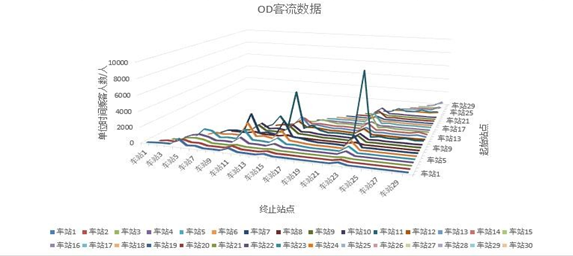
\includegraphics[scale=0.5]{OD客流数据.png}
	\caption{OD客流数据}
\end{figure}
由层次分析法得到各个站点的权值,依据权值大小来确定乘客人数高谷站点,因此可优先选择先发行覆盖于次站点的列车,即可减少乘客的候车时间,增加乘客的在车时间,及时满足乘客的需求,使服务水平最大化, 同时依据列车交替开行的运营模式(通常为1:n或n:1两种模式),则尽可能的均分大交路列车和小交路列车,制定合理组合,最后再考虑时间安全间隔,得到列车发行的时刻表。\par
写程序设计如图2。\par
\begin{figure}[h]
	\centering
	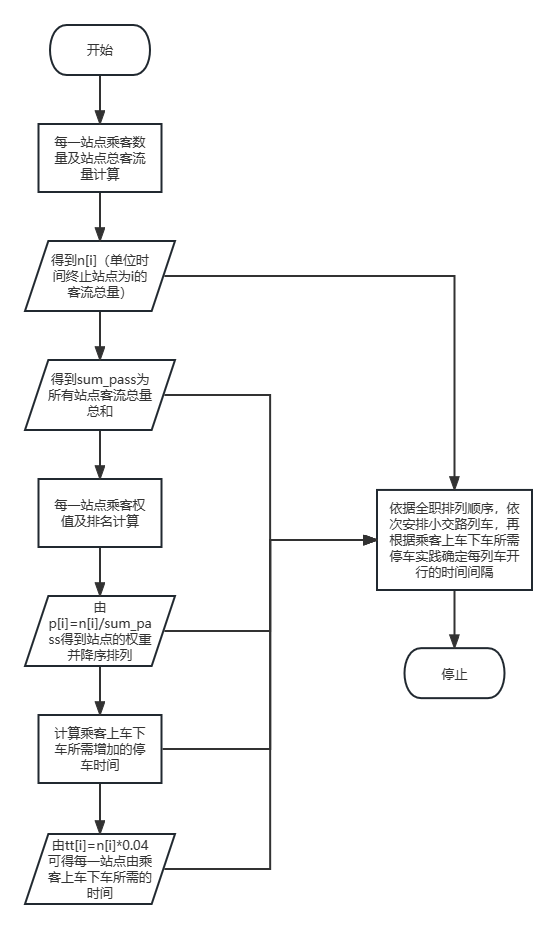
\includegraphics[scale=0.4]{模型二设计.png}
	\caption{模型二设计}
\end{figure}\par
根据列车的开行方案,计算每个车站的行车时间。这个时间包括列车进站时间、停车时间和列车出站时间。使用公式:\par
$$
t_{i,j}=\frac{d_{i,j}}{v}+s_i+p_i
$$\par
其中,$t_(i,j)$表示从站点i到站点j的行车时间,$d_(i,j)$表示站点i到站点j的距离,v表示列车的运行速度,$s_i$表示列车在站点i的进站时间,$p_i$表示列车在站点i的停车时间。\par
最后可以计算乘客的候车时间和乘车时间:\par
$$
w_i=\frac{1}{2}\cdot \frac{\sum_{j=1}^{i-1}{n_j}\cdot (t_i-t_{j,i})}{\sum_{j=1}^{i-1}{n_j}}
$$
$$
T_i=\frac{1}{2}\cdot \frac{\sum_{j=i+1}^n{n_j}\cdot (t_{j,i}-t_i)}{\sum_{j=i+1}^n{n_j}}
$$\par
其中,$w_i$表示在站点i等车的平均时间,$n_j$表示在站点j上车的乘客数量,$t_i$表示列车在站点i的到达时间,$t_(j,i)$表示从站点j到站点i的行车时间,$T_i$表示在站点i上车的平均时间,$n_j$表示在站点j上车的乘客数量,$t_i$表示列车在站点i的到达时间,$t_(j,i)$表示从站点j到站点i的行车时间。
\subsection{问题三}
由题目信息和附件5可知,问题一与问题二建立在原有的列车编组方案下,列车定员为1860(人/列)因此应改变列车类型及编组数量,增加列车定员,提升列车最大载客量(列车最大载客量即一个编制列车按车厢定员计算允许装载的最大乘客数),从而减少列车数量,降低乘客候车时间, 实现企业运营成本最小化和服务水平最大化目标,使得模型再次优化。\par
假定在新的列车编组方案施行下列车定员为2000(人/列)。\par
设$new\_big\_cnt$为新开行方案中大交路列车的数量,$new\_small\_cnt$为新开行方案中小交路每一站点的最小列车数量。\par
设$new\_big\_maxx$为大交路列车载客量,$new\_capacity$为列车最大载客量。\par
设原开行方案下大小交列车的总路程$s1$,新开行方案下大小交列车的总路程$s2$。\par
\section{模型求解}
\subsection{问题一的求解}
标记不具有折返能力的车站:\par
首先依据附件1可知车站数据,得到每一车站折返能力的属性,将不具有折返能力的车站标记为$true$,即若$i$为不具有折返能力的车站,则将$is\_not\left[ i \right] $标记为$true$,反之则标记为$false$。\par
即\par
$$
is\_not\left[ i \right] \left\{ \begin{array}{c}
	true\text{,车站}i\text{不具有折返能力}\\
	false\text{,车站}i\text{具有折返能力}\\
\end{array} \right. 
$$\par
大小交列车开行安排:\par
由附件4可知,车站1到车站30的最小断面客流量为3169人,最大客流量为46535人,如图4所示。
\begin{figure}[h]
	\centering
	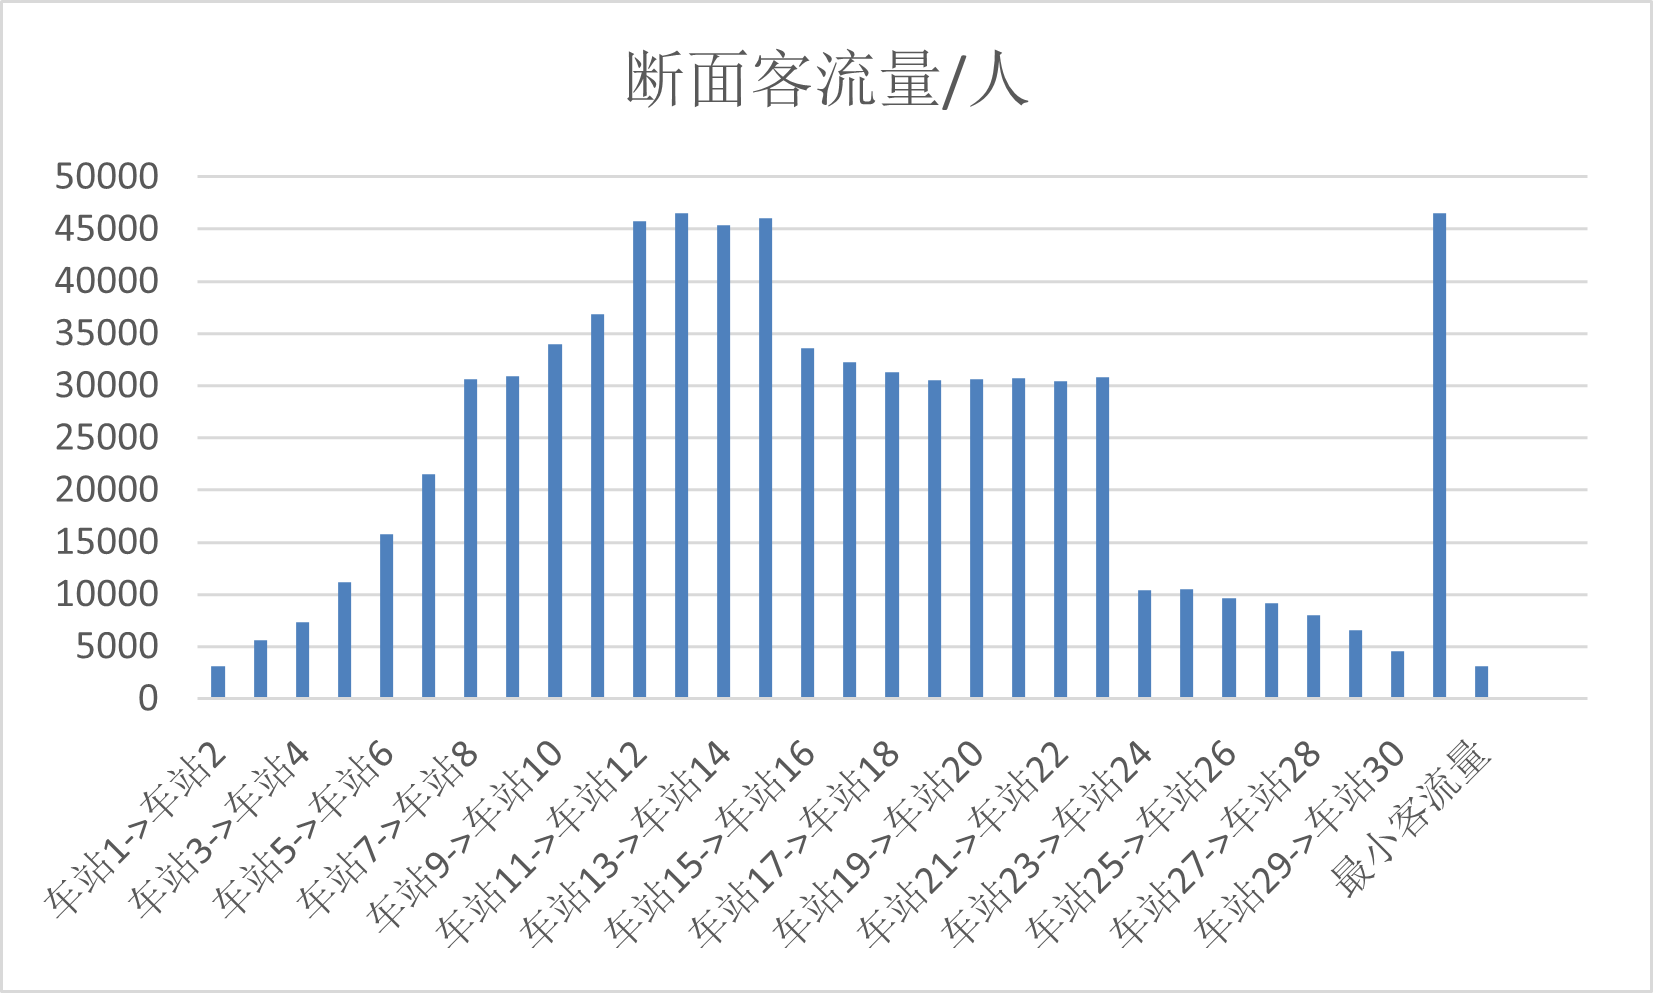
\includegraphics[scale=0.6]{断面客流量.png}
	\caption{断面客流量/人}
\end{figure}
则大交路列车安排开行数量为$\text{最小断面客流量}/\text{列车载客量}=3169/1860\text{列}$,向上取整为2列,同时各个站点减去大交路最大载客量$=\text{大交路列车开行数量}\times \text{列车载客量}=2\times 1860=3720\text{人}$,在与0去$max$得到每个站点在安排大交路列车后剩余要求负载的载客量。
即\par
$$
st\left[ i \right] =max\left( nums\left[ i \right] -big\_maxx,0 \right) \left( 1<=i<=30 \right) 
$$\par

每一站点更新数据如图5:\par
\begin{figure}[h]
	\centering
	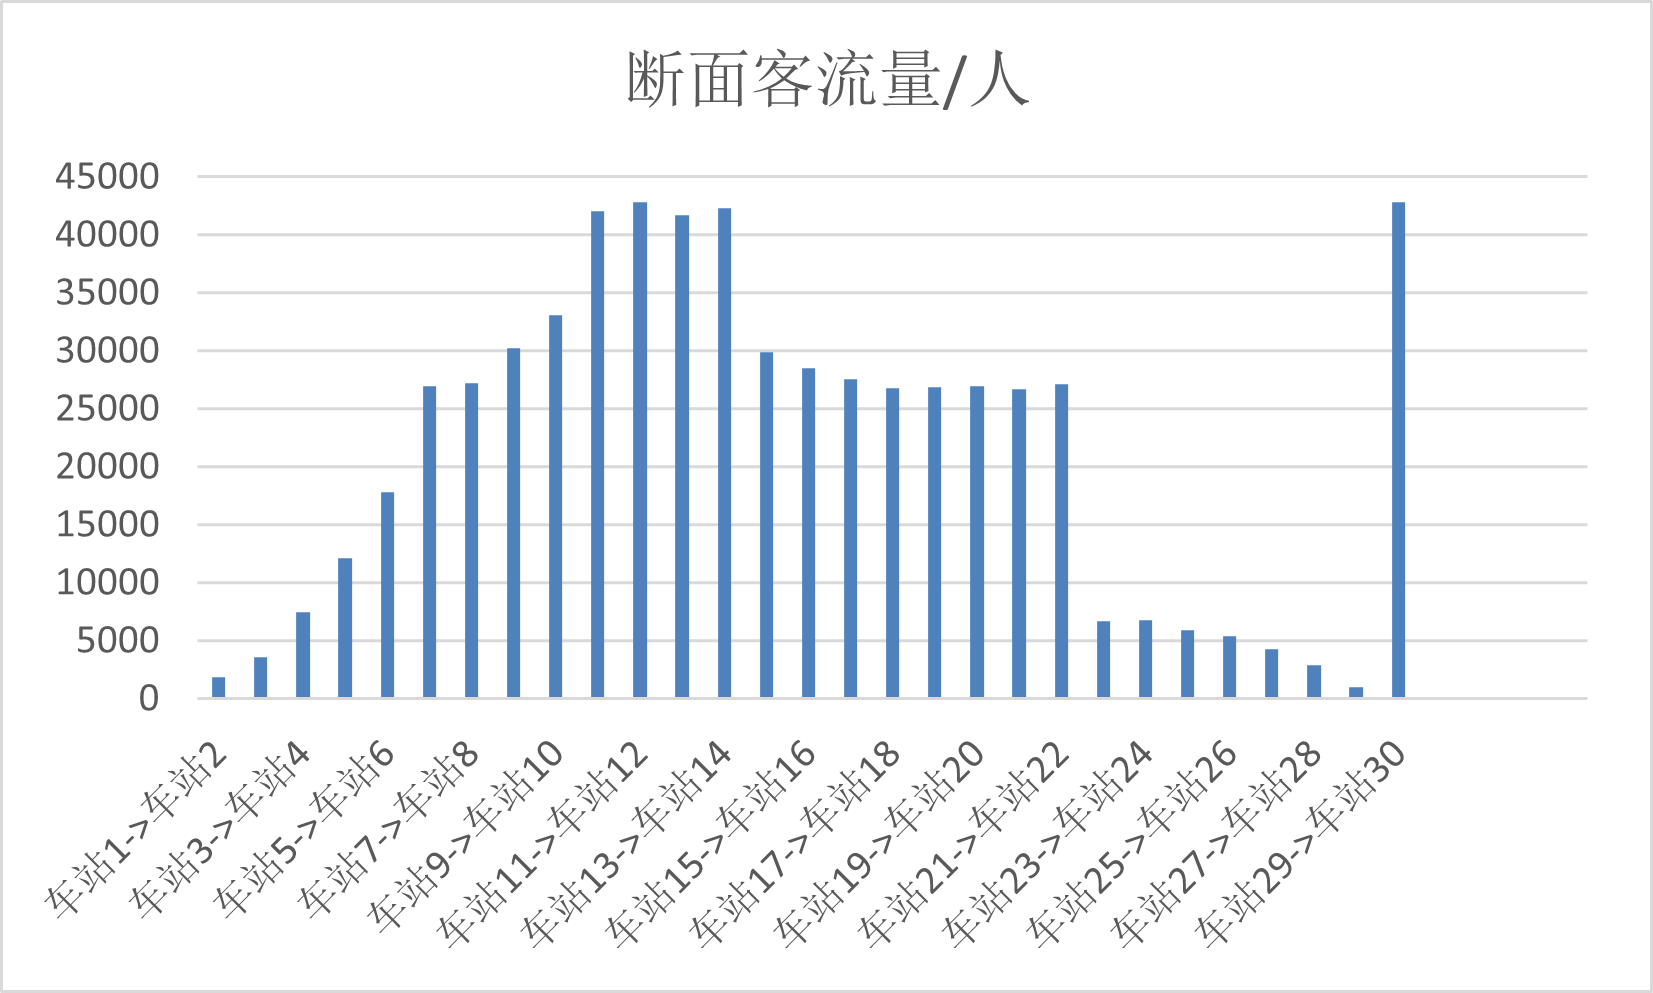
\includegraphics[scale=0.6]{更新站点断面客流量.png}
	\caption{更新站点断面客流量/人}
\end{figure}
则小交路列车在站点最大列车数量为最大断面客流量/列车载客量=42815/1860列,向上取整为24列,则第一次二分小交路列车的范围为[1,720]列,后再枚举小交路列车的运行区间长度,再写check 函数来判断设定小交路列车数量和运行区间长度的合理性。\par
具体步骤为:\par
1.使用设置完大交列车后,每一站点更新后所需断面客流量,计算出每一站点安排小交路列车向上取整时最小数量,同时用$must\_cnt$累加记录以列车数目为单位下的总客流量。
即\par
$$
\left\{ \begin{array}{c}
	small\_cnt\left[ i \right] =\left( st\left[ i \right] +big\_capacity \right) /big\_capacity,\left( 1<=i<=30 \right)\\
	must\_cnt=\sum_{i=1}^{i=30}{small\_cnt\left[ i \right]}\\
\end{array} \right. 
$$\par
2.第一次二分依据现实情况,缩小限定列车数量范围,由原来小交路列车数量范围为[1,720]改变到小交路列车区间通过车站数量范围设置为[3,24]后,将折半取中间值,代入下一次二分函数中,其中本次$binary\_two$判断函数为计算在小交列车数量为$mid$时,线路所能负载的客流总量,若满足或超过所要求负载的客流总量,则列车数量可以减少,列车选择范围为[l,mid];反之,则列车数量必须增加,列车选择范围为[mid+1,r];\par
3.第二次二分依据现实情况,缩小限定列车开行区间长度范围,由原来小交路列车开行区间范围为[1,30]调整为[2,4],将折半取中间值,代入check 判断函数为计算当小交路列车数量为$cnt$,开行区间为$mid$时,返回原计划小交路列车分配后剩余车辆数量,若原计划小交路列车分配后剩余车辆数量大于0则,列车开行区间可以减少,列车开行区间范围为[l,mid]; 反之,则列车开行区间必须增加,列车开行范围为[mid+1,r];\par
4.check判断函数中代入值为小交列车的数量和小交列车的开行区间,已知这两个信息后,由贪心算法的思想,将站名顺序遍历,后选择起点终点都为具备折返能力的车站,每次遇见第一个小于要求最小小交路列车要求数量,则在此处增加小交路列车数量,并将小交路列车原计划数量减少一个单位,后再更新区间长度为$len$的车站站点已承载客流量。\par
即\par
$$
\left\{ \begin{array}{c}
	1<=i<=30\\
	if\left( vis\left[ i \right] <small\_cnt\left[ i \right] \right) \\
	cur=\sum_{j=i+!}^{j<i+len\&\&j<30}{\max \left( small\_cnt\left[ j \right] -vis\left[ j \right] ,0 \right)}\\
	vis\left[ j \right] =\max \left( small\_cnt\left[ j \right] ,vis\left[ j \right] \right) \left( j<i+len\&\&j<30 \right)\\
\end{array} \right. 
$$\par
check 判断函数 C++代码见附录3。\par
5.输出每一站点的小交路列车的起始点,数量,输出结果如下表1。\par

\begin{table}[h!]
	\begin{center}
		\caption{问题一方案结果}
		\begin{tabular}{l|c|r|r} 
			  & \textbf{运行区间} & \textbf{运营里程} & \textbf{开行数量}\\
			\hline
			大交路 & 1站-30站 & 80.336 & 2列 \\
			小交路 & 2站-7站 & 64.73 & 10列 \\
			小交路 & 7站-13站 & 227.52 & 24列\\
			小交路 & 13站-19站 & 205.39 & 23列 \\
			小交路 & 19站-24站 & 96.21  & 15列 \\ 
			小交路 & 24站-30站 & 29.964 & 4列 \\
			
		\end{tabular}
	\end{center}
\end{table}
\subsection{问题二的求解}
由模型一可知,小交路列车安排数为5个区间,区间长度为5,各个站点发行数量分别为10,24,23,15,4。大交路列车安排发行数量为 2,则尽可能均分列车数目,得到两个分组为:\par
$$
\text{第一组为} 1\text{:}\left( 5+12+12+8+2 \right) =1:39
\\
\text{第二组为} 1\text{:}\left( 5+12+11+7+2 \right) =1:39
$$\par
每一站点乘客数量及站点总客流量计算:\par
由附件 3 可知,将终止车站的所有数据累加起来得到到达该站的单位时间总客流量。\par
即\par
$$
\left\{ \begin{array}{c}
	n\left[ i \right] =\sum_{j=1}^{j=29}{\sum_{i=2}^{i=30}{num\left[ j \right] \left[ i \right]}}\\
	sum\_pass=\sum_{i=2}^{i=30}{n\left[ i \right]}\\
\end{array} \right. 
$$\par
每一站点乘客权值及排名计算:\par
由上一步计算的每一站点乘客数量及站点总客流量值依据计算公式, 权值等于每一站点乘客数量除以站点总客流量,同时以降序排列则为各个站点的权值排名。\par
即\par
$$
p\left[ i \right] =nm\left[ i \right] /sum\_pass
$$\par
每一站点由乘客上下车所用的时间:\par
由附件 5 及题意可知,乘客平均上下时间为 0.04s,同时停车时间与乘客人数成正比,则停车时间为该站点乘客人数x 乘客平均上下时间。\par
即\par
$$
tt\left[ i \right] =n\left[ i \right] *0.04\left( 1<=i<=30 \right) 
$$\par
后依据模型一所得结果,将依次分配两个分组列车,同时按照权值优先分配列车,依据权值一一匹配最优时刻安排。\par
得到小交路列车开行方案如图6。
\begin{figure}[h]
	\centering
	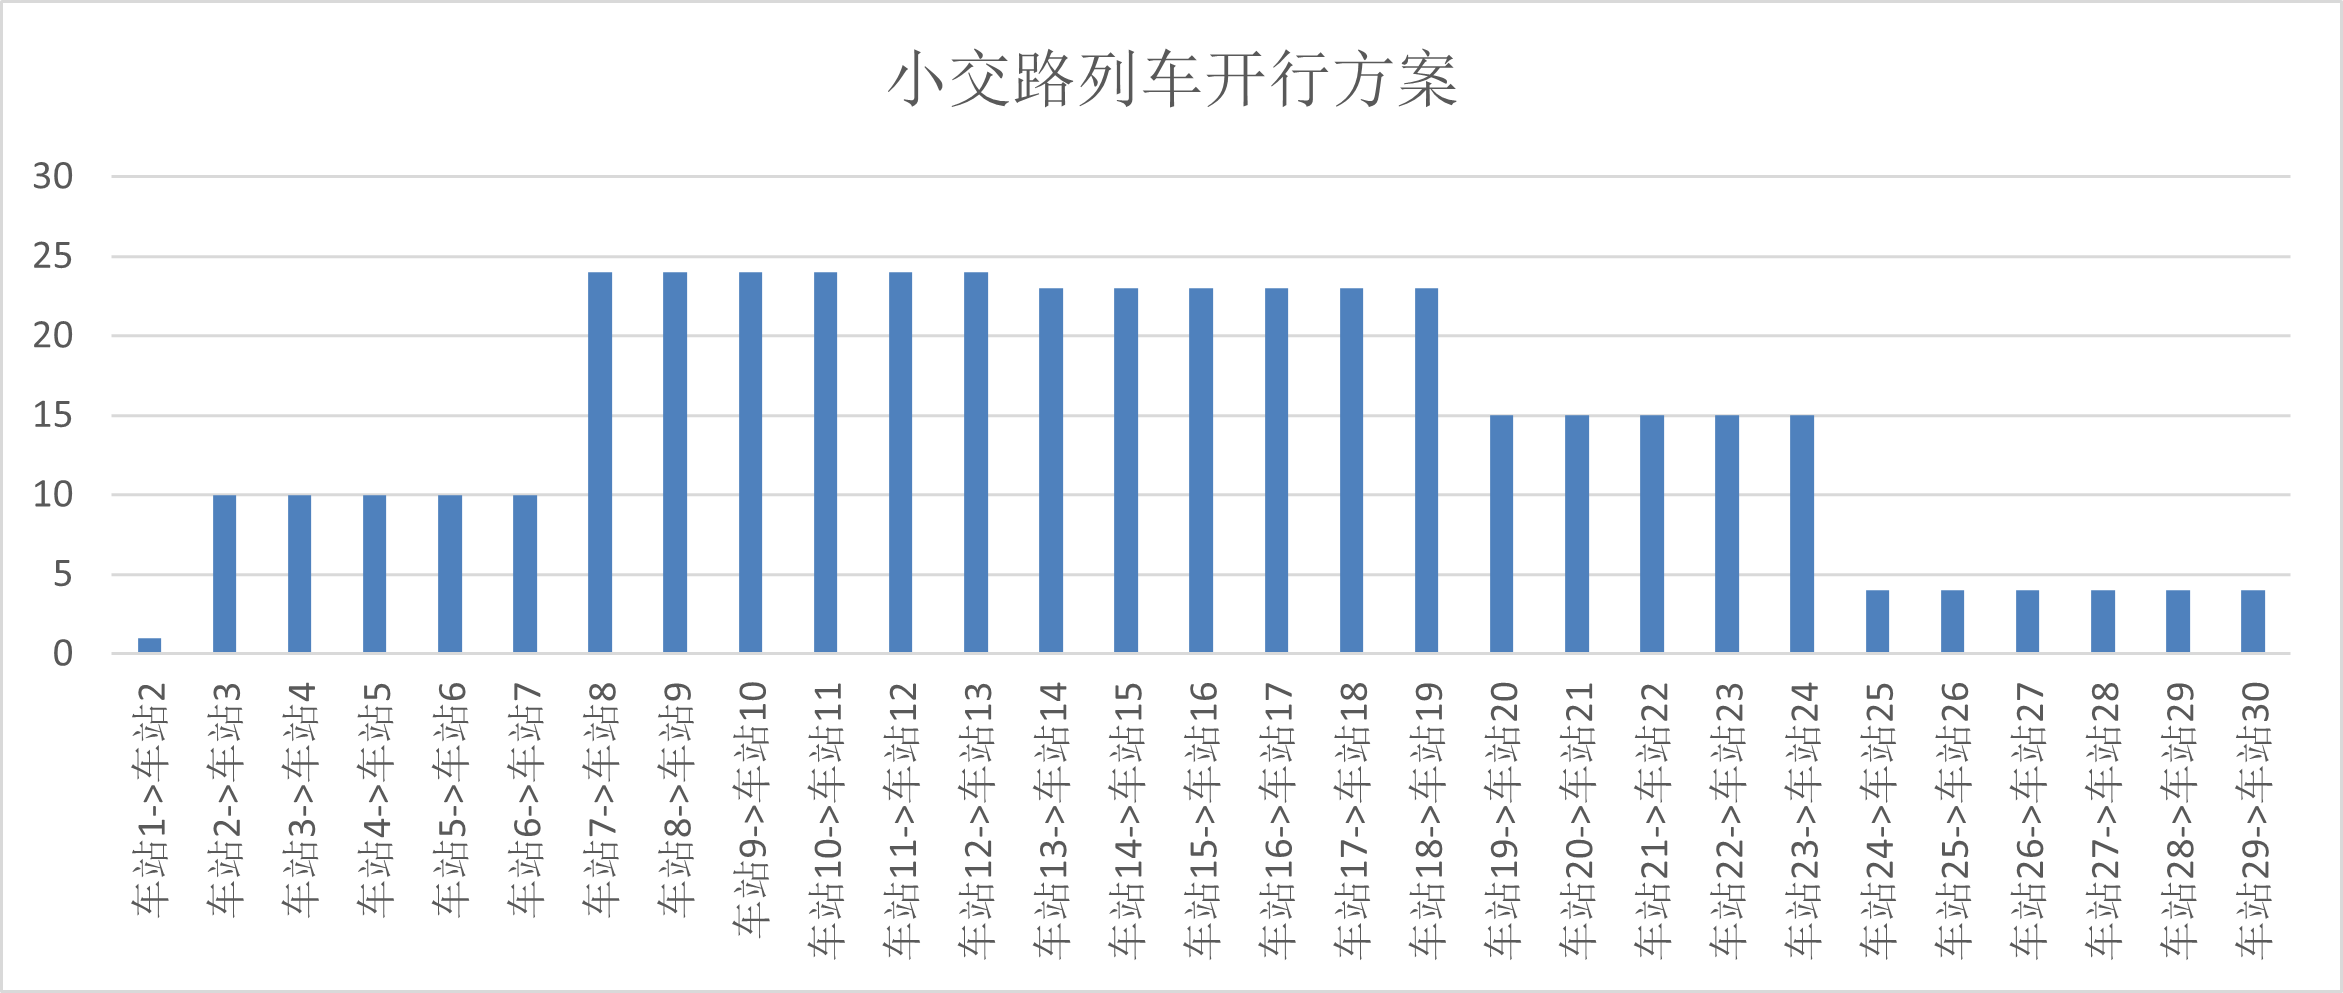
\includegraphics[scale=1]{小交路列车开行方案.png}
	\caption{小交路列车开行方案}
\end{figure}\par
计算权值排名运行结果为:\par 22,14,10,29,16,6,5,11,28,27,24,15,13,12,4,17,8,26,9,19,25,7,20,21,18,23,3,2,1。\par
1.先发行的小交路列车为从车站19开始的列车,列车数量为15,则站点19列车乘客上下所需停车总时间为tt[19]/15=1.6s,站点20列车乘客上下所需停车总时间为tt[20]/15=3.2s,站点21列车乘客上下所需停车总时间为tt[21]/15=2.4s,站点22列车乘客上下所需总停车时间为 tt[22]/15=1.7s, 站点23列车乘客上下所需总停车时间为tt[23]/15=62.3s。\par
	\begin{center}
	\begin{tabular}{c|c|c|c|c|c} 
		车站站点 & 19 & 20 & 21 & 22 & 23 \\
		\hline
		由乘客上下车所需停车总时 间(秒) & 1.6s & 3.2s & 2.4s & 1.7s & 62.3s \\	
	\end{tabular}
\end{center}\par
2.发行的小交路列车为从车站13开始的列车,列车数量为23,则站点13列车乘客上下所需停车总时间为tt[13]/23=3.9s,站点14列车乘客上下所需停车总时间为 tt[14]/23=28.1s,站点15列车乘客上下所需停车总时间为tt[15]/23=4.0s,站点16列车乘客上下所需总停车时间为 tt[16]/23=6.0s, 站点17列车乘客上下所需总停车时间为tt[17]/23=3.1s,站点 18列车乘客上下所需总停车时间为 tt[18]/23=1.0s。\par
	\begin{center}
	\begin{tabular}{c|c|c|c|c|c|c} 
		车站站点 & 13 & 14 & 15 & 16 & 17 & 18 \\
		\hline
		由乘客上下车所需停车总时 间(秒) & 3.9s & 28.1s & 4.0s & 6.0s & 3.1s & 1.0s \\	
	\end{tabular}
\end{center}\par
3.发行的小交路列车为从车站24开始的列车,列车数量为 4,则站点24列车乘客上下所需停车总时间为tt[24]/4=23.1s,站点25列车乘客上下所需停车总时间为 tt[25]/4=11.79s,站点26列车乘客上下所需停车总时间为tt[26]/4=13.86s,站点27列车乘客上下所需总停车时间为tt[27]/4=23.1s,站点28列车乘客上下所需总停车时间为tt[28]/4=23.3s,站点29列车乘客上下所需总时间为tt[29]/4=45.97s。\par
	\begin{center}
	\begin{tabular}{c|c|c|c|c|c|c} 
		车站站点 & 24 & 25 & 26 & 27 & 28 & 29 \\
		\hline
		由乘客上下车所需停车总时 间(秒) & 23.1s & 11.79s & 13.86s & 23.1s & 23.3s & 45.97s \\	
	\end{tabular}
\end{center}\par
4.发行的小交路列车为从车站 7 开始的列车,列车数量为24,则站点7列车乘客上下所需停车总时间为tt[7]/24=1.6s,站点8列车乘客上下所需停车总时间为 tt[8]/24=2.4s,站点9列车乘客上下所需停车总时间为tt[9]/24=2.2s,站点10列车乘客上下所需总停车时间为tt[10]/24=17.0s,站点11列车乘客上下所需总停车时间为tt[11]/24=3.8s,站点12列车乘客上下所需总时间为tt[12]/24=3.8s。\par
	\begin{center}
	\begin{tabular}{c|c|c|c|c|c|c} 
		车站站点 & 7 & 8 & 9 & 10 & 11 & 12 \\
		\hline
		由乘客上下车所需停车总时 间(秒) & 1.6s & 2.4s & 2.2s & 17.0s &3.8s & 3.8s \\	
	\end{tabular}
\end{center}\par
5.发行的小交路列车为从车站2开始的列车,列车数量为10,则站点2列车乘客上下所需停车总时间为tt[2]/10=1.5s,站点3列车乘客上下所需停车总时间为tt[3]/10=1.3s,站点4列车乘客上下所需总停车时间为tt[4]/10=9.0s,站点5列车乘客上下所需总停车时间为tt[5]/10=3.8s,站点6列车乘客上下所需总时间为tt[6]/10=10.1s。\par
	\begin{center}
	\begin{tabular}{c|c|c|c|c|c} 
		车站站点 & 2 & 3 & 4 & 5 & 6 \\
		\hline
		由乘客上下车所需停车总时 间(秒) & 1.5s & 1.3s & 9.0s & 3.8s & 10.1s \\	
	\end{tabular}
\end{center}\par
由开始确定分组列车数量均分特点可知,则第一分组站点列车所停车时间为停车总时间1/2,又由附件5可知,列车的追踪间隔时间为108s,停车范围为[20s,120s],因使最大化服务水平,则需最小化停车时间,将因乘客上下的停车时间与最小停车时间max值为真正的停车时间,再由所计算的停车时间和区间运行时间可得发车间隔时间,最终结果到计算结果。\par
\subsection{问题三的求解}
基于模型一的求解过程,将列车定员设置为2000(人/列)。\par
可以求得$new\_big\_cnt$为2列,新列车编组方案下小交路列车开行方案为\par
	\begin{center}
	\begin{tabular}{c|c} 
		\textbf{列车运行站点区间} & \textbf{列车开行列数} \\
		\hline
		车站2-车站7 & 6 列 \\
		车站7-车站13 & 15 列 \\
		车站13-车站19 & 12 列 \\
		车站19-车站24 & 9 列 \\
		车站24-车站30 & 2 列 \\
	\end{tabular}
\end{center}\par
得到\par
$$
S1=704.15km
$$
$$
S2=441.242km
$$\par
可知,与原列车编组方案,和模型一的最优解相比,优化了 37.34\%, 优化效果显著,因此所提出新列车编组方案具有有效性。
除此之外,针对降低企业运营成本和提高服务水平的问题,我们团队提出了以下一些方法和建议:\par
1.调整列车运行方案\par
通过对客流和车站数据的分析,我们可以发现有些站点的客流量较大,而有些站点的客流量较小,因此可以根据客流情况,调整列车运行方案,减少对客流量较小的站点的停靠次数,从而降低运营成本。另外,也可以采用智能调度算法,根据客流实时情况,调整列车运行方案,从而提高服务水平。\par
2.优化站点布局\par
通过对客流和车站数据的分析,我们可以发现有些站点之间的距离较短,可以考虑将这些站点合并,从而降低运营成本。另外,也可以优化站点的布局,使得客流量较大的站点能够更好地服务乘客,从而提高服务水平。\par
3.推广智能客流管理系统\par
智能客流管理系统可以通过采集和分析客流数据,实现客流预测和调度优化,从而降低运营成本和提高服务水平。因此,我们可以考虑在地铁系统中推广智能客流管理系统,以提高运营效率和服务水平。\par
4.加强智能安全监控\par
在地铁运营过程中,安全是至关重要的。因此,可以加强智能安全监控系统的建设,通过人脸识别等技术手段,实现对乘客和地铁设备的智能监控,从而提高运营安全和服务水平。\par
通过以上方法和建议,可以实现降低企业运营成本和提高服务水平的目标。同时,通过对客流和车站数据的量化分析支持,可以更好地指导地铁系统的运营和管理。\par

\section{模型的检验}
假设全部安排为大交列车下,列车数量由断面客流量最大站点决定,列车个数为46535/1860=26列(上取整结果)则运行里程数为26x80.336=1044.368km。则应用模型一方案,优化了32.58\%,应用模型三方案,优化了57.75\%。 \par
假设全部安排为区间长度为5的小交路列车下,列车数量由各个区间下最大断面客流量决定,列车安排方案为: \par
	\begin{center}
	\begin{tabular}{c|c} 
		\textbf{列车运行站点区间} & \textbf{列车开行列数} \\
		\hline
		车站1-车站5 & 7 列 \\
		车站5-车站10 & 19 列 \\
		车站10-车站15 & 26 列 \\
		车站15-车站20 & 19 列 \\
		车站20-车站25 & 17 列 \\
		车站25-车站30 & 6 列 \\
	\end{tabular}
\end{center}\par
则此此假设下列车行程总里数为 977.32km ,则应用模型一方案,优化了 27.94\%,应用模型三方案,优化了54.86\%。优化效果显著,则结果如图8所示。证明了本文所提出的模型方案的可行性与科学性。 \par
\begin{thebibliography}{40}
	\bibitem{ref1}赵丽红.基于遗传算法的公交车调度优化问题的研究[D].内蒙古大学,2010,12(02):04-22.
	\bibitem{ref2}邓连波,段科屹,汪晴等.城市轨道交通节能列车时刻表优化方法[J].系统工程理论与实践,2021,41(06):03-69.
	\bibitem{ref3}李莹,陈阳舟,詹璟原.基于动态客流的城市轨道列车全天时刻表优化[J].交通科技与经济,2019,21(05):42-53.
	\bibitem{ref4}蔡章辉,庞明宝,刁化尧.动态客流需求下城市轨道交通列车时刻表优化[J].铁道运输与经济,2017,39(01):07-16.
	\bibitem{ref5}胡三根,何琪,林锐浩.公交站点停靠时间及影响因素分析[J].、《广东工业大学学报》,2019,04(11):05-11.
	\bibitem{ref6}郑强.城市轨道交通地下线预制板式轨道研究及应用[J].城市轨道交通研究,2021,24(05):31-36.
	\bibitem{ref7}Doe,J. (2001). Train scheduling issues. In J. Rowell (Ed.), Essays on psychology (pp. 24-38). New York: Big Time Publisher.
	\bibitem{ref8}Smith, R., Orion, D. \& Johnson, S. Q. (2011, July 15). Bone-Chilling: Train parking scheme.In A. Hoffman \& C. G. Brooke (Eds.), Train literature through the ages (pp. 102-118). New York: Big Time Publisher.
	
	
	
	
\end{thebibliography}
\newpage
\newgeometry{left=1.50cm,right=0.5cm,top=3.00cm,bottom=3.0cm}	%修改附录代码的几何页面

\begin{center}
	\sihao \heiti 附录1
	\fontsize{10pt}{16pt}		\selectfont	
	\begin{lstlisting}[ 
		%C++程序代码
		language=C++,numbers=left,numberstyle=\tiny,keywordstyle=\color{blue!70},commentstyle=\color{red!50!green!50!blue!50},frame=shadowbox, rulesepcolor=\color{red!20!green!20!blue!20},escapeinside=``,xleftmargin=2em,xrightmargin=2em,aboveskip=1em] 
		//数据预处理C++程序代码
		#include<bits/stdc++.h>
		using
		namespace
		std;
		const
		int
		station_cnt = 30;//站点数量
		double
		as[station_cnt + 1];//相邻站间距/时间区间
		double
		os[station_cnt + 1];//任意站点到车站1的站间距/时间区间
		double
		ss[station_cnt + 1][station_cnt + 1];//任意两处车站点站间距/ 时间区间
		int main() {
			for (int
			i = 1; i < station_cnt; i++) {
				cin >> as[i];
			}
			for (int
			i = 1; i < station_cnt; i++) {
				os[i] += as[i] + os[i - 1];
			}
			for (int
			i = 0; i < station_cnt; i++) {
				for (int
				j = i + 1; j < station_cnt; j++) {
					ss[i][j] = os[j] - os[i];
				}
			}
			for (int
			i = 0; i < station_cnt; i++) {
				for (int
				j = i + 1; j < station_cnt; j++) {
					printf("车站%d->车站%d , %.0f\n", i + 1, j + 1, ss[i][j]);
				}
			}
			return 0;
		}
		
	\end{lstlisting}
\end{center}
\begin{center}
	\sihao \heiti 附录2
	
	
	\fontsize{10pt}{16pt}		\selectfont	
	\begin{lstlisting}[ 
		%C++程序代码
		language=C++,numbers=left,numberstyle=\tiny,keywordstyle=\color{blue!70},commentstyle=\color{red!50!green!50!blue!50},frame=shadowbox, rulesepcolor=\color{red!20!green!20!blue!20},escapeinside=``,xleftmargin=2em,xrightmargin=2em,aboveskip=1em] 
	//站点预处理后结果
	车站1与车站2的运行时间为:120
	车站1与车站3的运行时间为:121
	车站1与车站4的运行时间为:218
	车站1与车站5的运行时间为:220
	车站1与车站6的运行时间为:321
	车站1与车站7的运行时间为:322
	车站1与车站8的运行时间为:411
	车站1与车站9的运行时间为:412
	车站1与车站10的运行时间为:514
	车站1与车站11的运行时间为:515
	车站1与车站12的运行时间为:659
	车站1与车站13的运行时间为:661
	车站1与车站14的运行时间为:790
	车站1与车站15的运行时间为:791
	车站1与车站16的运行时间为:953
	车站1与车站17的运行时间为:956
	车站1与车站18的运行时间为:1059
	车站1与车站19的运行时间为:1060
	车站1与车站20的运行时间为:1156
	车站1与车站21的运行时间为:1157
	车站1与车站22的运行时间为:1296
	车站1与车站23的运行时间为:1297
	车站1与车站24的运行时间为:1430
	车站1与车站25的运行时间为:1432
	车站1与车站26的运行时间为:1514
	车站1与车站27的运行时间为:1515
	车站1与车站28的运行时间为:1609
	车站1与车站29的运行时间为:1610
	车站1与车站30的运行时间为:1803
	车站2与车站3的运行时间为:1
	车站2与车站4的运行时间为:98
	车站2与车站5的运行时间为:100
	车站2与车站6的运行时间为:201
	车站2与车站7的运行时间为:202
	车站2与车站8的运行时间为:291
	车站2与车站9的运行时间为:292
	车站2与车站10的运行时间为:394
	车站2与车站11的运行时间为:395
	车站2与车站12的运行时间为:539
	车站2与车站13的运行时间为:541
	车站2与车站14的运行时间为:670
	车站2与车站15的运行时间为:671
	车站2与车站16的运行时间为:833
	车站2与车站17的运行时间为:836
	车站2与车站18的运行时间为:939
	车站2与车站19的运行时间为:940
	车站2与车站20的运行时间为:1036
	车站2与车站21的运行时间为:1037
	车站2与车站22的运行时间为:1176
	车站2与车站23的运行时间为:1177
	车站2与车站24的运行时间为:1310
	车站2与车站25的运行时间为:1312
	车站2与车站26的运行时间为:1394
	车站2与车站27的运行时间为:1395
	车站2与车站28的运行时间为:1489
	车站2与车站29的运行时间为:1490
	车站2与车站30的运行时间为:1683
	车站3与车站4的运行时间为:97
	车站3与车站5的运行时间为:98
	车站3与车站6的运行时间为:199
	车站3与车站7的运行时间为:200
	车站3与车站8的运行时间为:289
	车站3与车站9的运行时间为:290
	车站3与车站10的运行时间为:392
	车站3与车站11的运行时间为:394
	车站3与车站12的运行时间为:538
	车站3与车站13的运行时间为:539
	车站3与车站14的运行时间为:668
	车站3与车站15的运行时间为:670
	车站3与车站16的运行时间为:832
	车站3与车站17的运行时间为:834
	车站3与车站18的运行时间为:937
	车站3与车站19的运行时间为:938
	车站3与车站20的运行时间为:1034
	车站3与车站21的运行时间为:1035
	车站3与车站22的运行时间为:1174
	车站3与车站23的运行时间为:1176
	车站3与车站24的运行时间为:1309
	车站3与车站25的运行时间为:1311
	车站3与车站26的运行时间为:1393
	车站3与车站27的运行时间为:1394
	车站3与车站28的运行时间为:1488
	车站3与车站29的运行时间为:1489
	车站3与车站30的运行时间为:1682
	车站4与车站5的运行时间为:1
	车站4与车站6的运行时间为:102
	车站4与车站7的运行时间为:103
	车站4与车站8的运行时间为:192
	车站4与车站9的运行时间为:193
	车站4与车站10的运行时间为:295
	车站4与车站11的运行时间为:297
	车站4与车站12的运行时间为:441
	车站4与车站13的运行时间为:442
	车站4与车站14的运行时间为:571
	车站4与车站15的运行时间为:573
	车站4与车站16的运行时间为:735
	车站4与车站17的运行时间为:737
	车站4与车站18的运行时间为:840
	车站4与车站19的运行时间为:841
	车站4与车站20的运行时间为:937
	车站4与车站21的运行时间为:938
	车站4与车站22的运行时间为:1077
	车站4与车站23的运行时间为:1079
	车站4与车站24的运行时间为:1212
	车站4与车站25的运行时间为:1214
	车站4与车站26的运行时间为:1296
	车站4与车站27的运行时间为:1297
	车站4与车站28的运行时间为:1391
	车站4与车站29的运行时间为:1392
	车站4与车站30的运行时间为:1585
	车站5与车站6的运行时间为:101
	车站5与车站7的运行时间为:102
	车站5与车站8的运行时间为:191
	车站5与车站9的运行时间为:192
	车站5与车站10的运行时间为:294
	车站5与车站11的运行时间为:295
	车站5与车站12的运行时间为:439
	车站5与车站13的运行时间为:441
	车站5与车站14的运行时间为:570
	车站5与车站15的运行时间为:572
	车站5与车站16的运行时间为:734
	车站5与车站17的运行时间为:736
	车站5与车站18的运行时间为:839
	车站5与车站19的运行时间为:840
	车站5与车站20的运行时间为:936
	车站5与车站21的运行时间为:937
	车站5与车站22的运行时间为:1076
	车站5与车站23的运行时间为:1078
	车站5与车站24的运行时间为:1211
	车站5与车站25的运行时间为:1213
	车站5与车站26的运行时间为:1295
	车站5与车站27的运行时间为:1296
	车站5与车站28的运行时间为:1390
	车站5与车站29的运行时间为:1391
	车站5与车站30的运行时间为:1584
	车站6与车站7的运行时间为:1
	车站6与车站8的运行时间为:90
	车站6与车站9的运行时间为:91
	车站6与车站10的运行时间为:193
	车站6与车站11的运行时间为:194
	车站6与车站12的运行时间为:338
	车站6与车站13的运行时间为:340
	车站6与车站14的运行时间为:469
	车站6与车站15的运行时间为:471
	车站6与车站16的运行时间为:633
	车站6与车站17的运行时间为:635
	车站6与车站18的运行时间为:738
	车站6与车站19的运行时间为:739
	车站6与车站20的运行时间为:835
	车站6与车站21的运行时间为:836
	车站6与车站22的运行时间为:975
	车站6与车站23的运行时间为:977
	车站6与车站24的运行时间为:1110
	车站6与车站25的运行时间为:1112
	车站6与车站26的运行时间为:1194
	车站6与车站27的运行时间为:1195
	车站6与车站28的运行时间为:1289
	车站6与车站29的运行时间为:1290
	车站6与车站30的运行时间为:1483
	车站7与车站8的运行时间为:89
	车站7与车站9的运行时间为:90
	车站7与车站10的运行时间为:192
	车站7与车站11的运行时间为:193
	车站7与车站12的运行时间为:337
	车站7与车站13的运行时间为:339
	车站7与车站14的运行时间为:468
	车站7与车站15的运行时间为:470
	车站7与车站16的运行时间为:632
	车站7与车站17的运行时间为:634
	车站7与车站18的运行时间为:737
	车站7与车站19的运行时间为:738
	车站7与车站20的运行时间为:834
	车站7与车站21的运行时间为:835
	车站7与车站22的运行时间为:974
	车站7与车站23的运行时间为:976
	车站7与车站24的运行时间为:1109
	车站7与车站25的运行时间为:1110
	车站7与车站26的运行时间为:1192
	车站7与车站27的运行时间为:1193
	车站7与车站28的运行时间为:1287
	车站7与车站29的运行时间为:1288
	车站7与车站30的运行时间为:1481
	车站8与车站9的运行时间为:1
	车站8与车站10的运行时间为:103
	车站8与车站11的运行时间为:104
	车站8与车站12的运行时间为:248
	车站8与车站13的运行时间为:250
	车站8与车站14的运行时间为:379
	车站8与车站15的运行时间为:381
	车站8与车站16的运行时间为:543
	车站8与车站17的运行时间为:545
	车站8与车站18的运行时间为:648
	车站8与车站19的运行时间为:649
	车站8与车站20的运行时间为:745
	车站8与车站21的运行时间为:746
	车站8与车站22的运行时间为:885
	车站8与车站23的运行时间为:887
	车站8与车站24的运行时间为:1020
	车站8与车站25的运行时间为:1021
	车站8与车站26的运行时间为:1103
	车站8与车站27的运行时间为:1104
	车站8与车站28的运行时间为:1198
	车站8与车站29的运行时间为:1199
	车站8与车站30的运行时间为:1392
	车站9与车站10的运行时间为:102
	车站9与车站11的运行时间为:103
	车站9与车站12的运行时间为:247
	车站9与车站13的运行时间为:249
	车站9与车站14的运行时间为:378
	车站9与车站15的运行时间为:380
	车站9与车站16的运行时间为:542
	车站9与车站17的运行时间为:544
	车站9与车站18的运行时间为:647
	车站9与车站19的运行时间为:648
	车站9与车站20的运行时间为:744
	车站9与车站21的运行时间为:745
	车站9与车站22的运行时间为:884
	车站9与车站23的运行时间为:886
	车站9与车站24的运行时间为:1019
	车站9与车站25的运行时间为:1021
	车站9与车站26的运行时间为:1103
	车站9与车站27的运行时间为:1103
	车站9与车站28的运行时间为:1197
	车站9与车站29的运行时间为:1199
	车站9与车站30的运行时间为:1392
	车站10与车站11的运行时间为:1
	车站10与车站12的运行时间为:145
	车站10与车站13的运行时间为:147
	车站10与车站14的运行时间为:276
	车站10与车站15的运行时间为:278
	车站10与车站16的运行时间为:440
	车站10与车站17的运行时间为:442
	车站10与车站18的运行时间为:545
	车站10与车站19的运行时间为:546
	车站10与车站20的运行时间为:642
	车站10与车站21的运行时间为:643
	车站10与车站22的运行时间为:782
	车站10与车站23的运行时间为:784
	车站10与车站24的运行时间为:917
	车站10与车站25的运行时间为:919
	车站10与车站26的运行时间为:1001
	车站10与车站27的运行时间为:1001
	车站10与车站28的运行时间为:1095
	车站10与车站29的运行时间为:1097
	车站10与车站30的运行时间为:1290
	车站11与车站12的运行时间为:144
	车站11与车站13的运行时间为:146
	车站11与车站14的运行时间为:275
	车站11与车站15的运行时间为:276
	车站11与车站16的运行时间为:438
	车站11与车站17的运行时间为:441
	车站11与车站18的运行时间为:544
	车站11与车站19的运行时间为:545
	车站11与车站20的运行时间为:641
	车站11与车站21的运行时间为:642
	车站11与车站22的运行时间为:781
	车站11与车站23的运行时间为:783
	车站11与车站24的运行时间为:916
	车站11与车站25的运行时间为:917
	车站11与车站26的运行时间为:999
	车站11与车站27的运行时间为:1000
	车站11与车站28的运行时间为:1094
	车站11与车站29的运行时间为:1095
	车站11与车站30的运行时间为:1288
	车站12与车站13的运行时间为:2
	车站12与车站14的运行时间为:131
	车站12与车站15的运行时间为:132
	车站12与车站16的运行时间为:294
	车站12与车站17的运行时间为:297
	车站12与车站18的运行时间为:400
	车站12与车站19的运行时间为:401
	车站12与车站20的运行时间为:497
	车站12与车站21的运行时间为:498
	车站12与车站22的运行时间为:637
	车站12与车站23的运行时间为:639
	车站12与车站24的运行时间为:772
	车站12与车站25的运行时间为:773
	车站12与车站26的运行时间为:855
	车站12与车站27的运行时间为:856
	车站12与车站28的运行时间为:950
	车站12与车站29的运行时间为:951
	车站12与车站30的运行时间为:1144
	车站13与车站14的运行时间为:129
	车站13与车站15的运行时间为:131
	车站13与车站16的运行时间为:293
	车站13与车站17的运行时间为:295
	车站13与车站18的运行时间为:398
	车站13与车站19的运行时间为:399
	车站13与车站20的运行时间为:495
	车站13与车站21的运行时间为:496
	车站13与车站22的运行时间为:635
	车站13与车站23的运行时间为:637
	车站13与车站24的运行时间为:770
	车站13与车站25的运行时间为:771
	车站13与车站26的运行时间为:853
	车站13与车站27的运行时间为:854
	车站13与车站28的运行时间为:948
	车站13与车站29的运行时间为:949
	车站13与车站30的运行时间为:1142
	车站14与车站15的运行时间为:2
	车站14与车站16的运行时间为:164
	车站14与车站17的运行时间为:166
	车站14与车站18的运行时间为:269
	车站14与车站19的运行时间为:270
	车站14与车站20的运行时间为:366
	车站14与车站21的运行时间为:367
	车站14与车站22的运行时间为:506
	车站14与车站23的运行时间为:508
	车站14与车站24的运行时间为:641
	车站14与车站25的运行时间为:642
	车站14与车站26的运行时间为:724
	车站14与车站27的运行时间为:725
	车站14与车站28的运行时间为:819
	车站14与车站29的运行时间为:820
	车站14与车站30的运行时间为:1013
	车站15与车站16的运行时间为:162
	车站15与车站17的运行时间为:164
	车站15与车站18的运行时间为:267
	车站15与车站19的运行时间为:269
	车站15与车站20的运行时间为:365
	车站15与车站21的运行时间为:366
	车站15与车站22的运行时间为:505
	车站15与车站23的运行时间为:506
	车站15与车站24的运行时间为:639
	车站15与车站25的运行时间为:641
	车站15与车站26的运行时间为:723
	车站15与车站27的运行时间为:724
	车站15与车站28的运行时间为:818
	车站15与车站29的运行时间为:819
	车站15与车站30的运行时间为:1012
	车站16与车站17的运行时间为:2
	车站16与车站18的运行时间为:105
	车站16与车站19的运行时间为:107
	车站16与车站20的运行时间为:203
	车站16与车站21的运行时间为:204
	车站16与车站22的运行时间为:343
	车站16与车站23的运行时间为:344
	车站16与车站24的运行时间为:477
	车站16与车站25的运行时间为:479
	车站16与车站26的运行时间为:561
	车站16与车站27的运行时间为:562
	车站16与车站28的运行时间为:656
	车站16与车站29的运行时间为:657
	车站16与车站30的运行时间为:850
	车站17与车站18的运行时间为:103
	车站17与车站19的运行时间为:104
	车站17与车站20的运行时间为:200
	车站17与车站21的运行时间为:201
	车站17与车站22的运行时间为:340
	车站17与车站23的运行时间为:342
	车站17与车站24的运行时间为:475
	车站17与车站25的运行时间为:477
	车站17与车站26的运行时间为:559
	车站17与车站27的运行时间为:559
	车站17与车站28的运行时间为:653
	车站17与车站29的运行时间为:655
	车站17与车站30的运行时间为:848
	车站18与车站19的运行时间为:1
	车站18与车站20的运行时间为:97
	车站18与车站21的运行时间为:98
	车站18与车站22的运行时间为:237
	车站18与车站23的运行时间为:239
	车站18与车站24的运行时间为:372
	车站18与车站25的运行时间为:374
	车站18与车站26的运行时间为:456
	车站18与车站27的运行时间为:456
	车站18与车站28的运行时间为:550
	车站18与车站29的运行时间为:552
	车站18与车站30的运行时间为:745
	车站19与车站20的运行时间为:96
	车站19与车站21的运行时间为:97
	车站19与车站22的运行时间为:236
	车站19与车站23的运行时间为:238
	车站19与车站24的运行时间为:371
	车站19与车站25的运行时间为:372
	车站19与车站26的运行时间为:454
	车站19与车站27的运行时间为:455
	车站19与车站28的运行时间为:549
	车站19与车站29的运行时间为:550
	车站19与车站30的运行时间为:743
	车站20与车站21的运行时间为:1
	车站20与车站22的运行时间为:140
	车站20与车站23的运行时间为:142
	车站20与车站24的运行时间为:275
	车站20与车站25的运行时间为:276
	车站20与车站26的运行时间为:358
	车站20与车站27的运行时间为:359
	车站20与车站28的运行时间为:453
	车站20与车站29的运行时间为:454
	车站20与车站30的运行时间为:647
	车站21与车站22的运行时间为:139
	车站21与车站23的运行时间为:141
	车站21与车站24的运行时间为:274
	车站21与车站25的运行时间为:275
	车站21与车站26的运行时间为:357
	车站21与车站27的运行时间为:358
	车站21与车站28的运行时间为:452
	车站21与车站29的运行时间为:453
	车站21与车站30的运行时间为:646
	车站22与车站23的运行时间为:2
	车站22与车站24的运行时间为:135
	车站22与车站25的运行时间为:136
	车站22与车站26的运行时间为:218
	车站22与车站27的运行时间为:219
	车站22与车站28的运行时间为:313
	车站22与车站29的运行时间为:314
	车站22与车站30的运行时间为:507
	车站23与车站24的运行时间为:133
	车站23与车站25的运行时间为:135
	车站23与车站26的运行时间为:217
	车站23与车站27的运行时间为:218
	车站23与车站28的运行时间为:312
	车站23与车站29的运行时间为:313
	车站23与车站30的运行时间为:506
	车站24与车站25的运行时间为:2
	车站24与车站26的运行时间为:84
	车站24与车站27的运行时间为:85
	车站24与车站28的运行时间为:179
	车站24与车站29的运行时间为:180
	车站24与车站30的运行时间为:373
	车站25与车站26的运行时间为:82
	车站25与车站27的运行时间为:83
	车站25与车站28的运行时间为:177
	车站25与车站29的运行时间为:178
	车站25与车站30的运行时间为:371
	车站26与车站27的运行时间为:1
	车站26与车站28的运行时间为:95
	车站26与车站29的运行时间为:96
	车站26与车站30的运行时间为:289
	车站27与车站28的运行时间为:94
	车站27与车站29的运行时间为:95
	车站27与车站30的运行时间为:288
	车站28与车站29的运行时间为:1
	车站28与车站30的运行时间为:194
	车站29与车站30的运行时间为:193
	\end{lstlisting}
\end{center}
\begin{center}
	\sihao \heiti 附录3
	
	
	\fontsize{10pt}{16pt}		\selectfont	
	\begin{lstlisting}[ 
		%C++程序代码
		language=C++,numbers=left,numberstyle=\tiny,keywordstyle=\color{blue!70},commentstyle=\color{red!50!green!50!blue!50},frame=shadowbox, rulesepcolor=\color{red!20!green!20!blue!20},escapeinside=``,xleftmargin=2em,xrightmargin=2em,aboveskip=1em] 
	//check 判断函数 C++代码
	pair<int,int> check(int cnt,int len){
		
		int cur=0;//将客流量以列车数量为单位,得到在列车数目为 cnt,区间长度为 len 下所承载的客流量的值
		
		unordered_map<int,int>vis;//已覆盖小交路列车个数for(int i = 1 ; i < 30 ; i++ ){
			if(is_not[i]&&((i+len<30&&is_not[i+len])||i+len>=30))continue;//不能作为小交路列车的起始终止点将被除去
			
			if(cnt==0)return {0,cur};//原计划的车辆列数为 0 时,返回当前所承载的用户量(用列车数量为单位)
			
			if(vis[i]<small_cnt[i]){//小于要求最小小交路列车要求数量,则在此处增加小交路
				列车数量
				
				cnt--;//第一次二分得出的个数,此处增加小交路列车数量,则原计划小交路列车数量减一(逆向思维)
				
				for(int j=i;j<=i+len&&j<30;j++){ cur+=max(small_cnt[j]-vis[j],0);//计算承载客流量
					vis[j]=max(small_cnt[j],vis[j]);//更新站点的车辆数目
					
				}
			}
		}
	\end{lstlisting}
\end{center}
\begin{center}
	\sihao \heiti 附录4
	
	
	\fontsize{10pt}{16pt}		\selectfont	
	\begin{lstlisting}[ 
		%问题一C++程序代码
		language=C++,numbers=left,numberstyle=\tiny,keywordstyle=\color{blue!70},commentstyle=\color{red!50!green!50!blue!50},frame=shadowbox, rulesepcolor=\color{red!20!green!20!blue!20},escapeinside=``,xleftmargin=2em,xrightmargin=2em,aboveskip=1em] 
		//数据预处理C++程序代码
		#include<bits/stdc++.h>
		using
		namespace
		std;
		const
		int
		big_maxx = 2 * 1860;//大交路载客量
		const
		int
		big_capacity = 1860;//列车的最大载客量
		int
		nums[50];//断面客流量
		int
		st[50];//更新站点客流量
		unordered_map<int, bool>is_not;//没有折返能力的车站
		int
		is_not_cnt;//没有折返能力的车站总数目
		int
		small_cnt[50];//每一站点所需小交路列车的数量
		int
		_num, _len;//小交路列车的数量,区间长度
		int
		must_cnt;//以列车数目为单位的总客流量
		pair<int, int>
		check(int
		cnt, int
		len) {
			int
			cur = 0;//将客流量以列车数量为单位,得到在列车数目为cnt,区间长度为
			len下所承载的客流量的值
			unordered_map<int, int>vis;//已覆盖小交路列车个数
			for (int
			i
			=
			1
			;
			i
			<
			30
			;
			i++
			) {
				if (is_not[i] && ((i + len < 30 && is_not[i + len]) || i + len >= 30))continue; /
				/不能作为小交路列车的起始终止点将被除去
				if (cnt == 0)return
				{ 0,cur };//原计划的车辆列数为0时,返回当前所承载的
				用户量(用列车数量为单位)
				if (vis[i] < small_cnt[i]) {//小于要求最小小交路列车要求数量,则在此处增
					加小交路列车数量
					cnt--;//第一次二分得出的个数,此处增加小交路列车数量,则原计划小交路
					列车数量减一(逆向思维)
					for (int
					j = i; j <= i + len && j < 30; j++) {
						cur += max(small_cnt[j] - vis[j], 0);//计算承载客流量
						vis[j] = max(small_cnt[j], vis[j]);//更新站点的车辆数目
					}
				}
			}
			return
			{ cnt,cur };
		}
		void
		print(int
		cnt, int
		len) {
			map<int, int>vis;//已覆盖小交路列车个数
			vector<int>vec;//列车开行方案
			for (int
			i = 1; i < 30; i++) {
				if (is_not[i] && ((i + len < 30 && is_not[i + len]) || i + len >= 30))continue; /
				/不能作为小交路列车的起始终止点将被除去
				if (vis[i] < small_cnt[i]) {//小于要求最小小交路列车要求数量,则在此处增
					加小交路列车数量
					vec.push_back(i);//记录车站站点
					for (int
					j = i; j <= i + len && j < 30; j++) {
						vis[j] = max(small_cnt[j], vis[j]);//更新站点的车辆数目
					}
				}
			}
			for (int
			i = 0; i < vec.size(); i++) {
				for (int
				j = vec[i]; j <= vec[i] + len && j < 30; j++) {
					vis[vec[i]] = max(vis[j], vis[vec[i]]);//更新每一开行区间中列车的数
					量
				}
			}
			cout << vec.size() << "个小交路公交站和区间长度为" << len + 1 << endl;
			for (auto
			it : vec) {
				cout << it << "站:" << vis[it] << endl;
			}
			puts("");
			return
			;
			int
			binary_two(int
			cnt) {
				int
				l = 2, r = 4;//限定开行区间长度范围
				while (l < r) {
					int
					mid = l + r >> 1;
					if (check(cnt, mid).first >= 0) {
						l = mid + 1;
					}
					else
					r = mid;
				}
				_len = l;
				return
				check(cnt, l).second;
			}
			void
			binary_one() {
				int
				l = 3, r = 24;//限定列车数量范围
				while (l < r) {
					int
					mid = l + r >> 1;
					if (binary_two(mid) >= must_cnt) {//满足
						r = mid;
					}
					else
					l = mid + 1;
				}
				_num = l;
			}
			int
			main() {
				for (int
				i = 1; i < 30; i++) {
					scanf("%d", &nums[i]);
				}
				cin >> is_not_cnt;
				for (int
				i = 1; i <= is_not_cnt; i++) {
					int
					node;
					cin >> node;
					is_not[node] = true;//将不能作为小交路列车的起点终点坐标标记
				}
				for (int
				i = 1; i < 30; i++) {
					st[i] = max(nums[i] - big_maxx, 0);
				}
				for (int
				i = 1; i < 30; i++) {
					small_cnt[i] = (st[i] + big_capacity - 1) / big_capacity;//每一站点小交
					路列车向上取整时最小数量
					must_cnt += small_cnt[i];//将总客流量换算为列车数目为单位
				}
				binary_one();
				print(_num, _len);
				return 0;
			}
	\end{lstlisting}
\end{center}
\begin{center}
	\sihao \heiti 附录5
	\fontsize{10pt}{16pt}		\selectfont	
	\begin{lstlisting}[ language=MATLAB,numbers=left,numberstyle=\tiny,keywordstyle=\color{blue!70},commentstyle=\color{red!50!green!50!blue!50},frame=shadowbox, rulesepcolor=\color{red!20!green!20!blue!20},escapeinside=``,xleftmargin=2em,xrightmargin=2em,aboveskip=1em] 
		%MATLAB问题一
		clc
		clear
		[~, ~, G] = xlsread('附件1:车站数据.xlsx');
		G = G(2:end,2); % 去除车站名称列
		T = xlsread('附件2:区间运行时间.xlsx');
		C = xlsread('附件3:OD客流数据.xlsx');
		D = xlsread('附件4:断面客流数据.xlsx');
		min_max_headway = [120, 360];
		min_spacing = 108;
		min_max_stop_time = [20, 120];
		train_capacity = 1860;
		min_max_station_num = [3, 24];
		avg_boarding_time = 0.04;
		
		n = size(T,1); % 大交路数量
		m = size(T,2); % 小交路数量
		
		f = [C(:); ones(m,1)]; % 目标函数系数
		
		Aeq = zeros(m, n*m + m); % 相等约束系数矩阵
		beq = D(:); % 相等约束右侧常数
		
		lb = zeros(n*m+m,1); % 变量下限
		
		% 不等约束系数矩阵
		A = zeros(m*n,n*m+m);
		b = zeros(m*n,1);
		
		% 相等约束
		for j = 1:m
		Aeq(j, (j-1)*n+1:j*n) = 1;
		Aeq(j, n*m+j) = 1;
		end
		
		% 不等约束
		for j = 1:m
		for i = 1:n
		A((j-1)*n+i, (i-1)*m+j) = 1;
		A((j-1)*n+i, n*m+j) = T(i,j);
		end
		A((j-1)*n+1:j*n, n*m+j) = -1;
		b((j-1)*n+1:j*n) = -min_max_headway(1) * D(j) / 3600; % 转换为小时
		end
		
		% 非负约束
		for i = 1:n*m+m
		lb(i) = 0;
		end
		
		% 上下界约束
		ub = Inf(n*m+m,1);
		for j = 1:m
		ub(n*m+j) = min_max_headway(2);
		end
		for i = 1:n
		for j = 1:m
		ub((i-1)*m+j) = min(D(j), train_capacity) / train_capacity;
		end
		end
		
		for j = 1:m
		station_num = 0; % 初始化车站数量为0
		for i = 1:n
		if G{i,j} == 1 % 统计车站数量
		station_num = station_num + 1;
		end
		end
		A((j-1)*n+1:j*n, (j-1)*n+1:j*n) = -station_num*avg_boarding_time*ones(n);
		b((j-1)*n+1:j*n) = -min_max_stop_time(1)*station_num*ones(n);
		end
		
		[x, ~, ~, ~] = linprog(f, A, b, Aeq, beq, lb, ub);
		
		% 提取解向量中的决策变量
		X = reshape(x(1:nm), n, m);
		Y = x(nm+1:n*m+m);
		
		% 打印结果
		fprintf('Objective Value: %f\n', fval);
		fprintf('X:\n');
		disp(X);
		fprintf('Y:\n');
		disp(Y);
	\end{lstlisting}
\end{center}
\begin{center}
	\sihao \heiti 附录6
	\fontsize{10pt}{16pt}		\selectfont	
	\begin{lstlisting}[ language=MATLAB,numbers=left,numberstyle=\tiny,keywordstyle=\color{blue!70},commentstyle=\color{red!50!green!50!blue!50},frame=shadowbox, rulesepcolor=\color{red!20!green!20!blue!20},escapeinside=``,xleftmargin=2em,xrightmargin=2em,aboveskip=1em] 
		%MATLAB问题二
	% 列名重命名过
	% 车站名称(station_name)	是否可作为交路起点/终点(if_origin_destination)
	% 区间(interval)	区间运行时间/s(running_time)	站间距/km(station_spacing)
	% 车站1-30 改为station_1到station_30
	
	% 读取车站数据
	station_data = readtable('附件1:车站数据.xlsx');
	is_start_end = strcmp(station_data.if_origin_destination, '是'); % 判断是否为起点或终点
	start_end_stations = station_data(is_start_end, :); % 起点和终点车站
	num_start_end = size(start_end_stations, 1); % 起点和终点车站数目
	
	% 读取区间运行时间
	interval_data = readtable('附件2:区间运行时间.xlsx');
	num_interval = size(interval_data, 1); % 区间数目
	
	% 读取OD客流数据
	od_data = readtable('附件3:OD客流数据.xlsx');
	num_station = size(od_data, 1); % 车站数目
	od_matrix = table2array(od_data(:, 2:end)); % 提取OD客流矩阵
	
	% 计算交路运行时间和运行里程
	route_time = zeros(num_start_end, num_start_end); % 交路运行时间矩阵
	route_distance = zeros(num_start_end, num_start_end); % 交路运行里程矩阵
	for i = 1:num_start_end
	for j = 1:num_start_end
	if i == j
	continue;
	end
	start_station = start_end_stations(i, :).station_name{1};
	end_station = start_end_stations(j, :).station_name{1};
	interval_index = strcmp(interval_data.interval, [start_station '->' end_station]);
	route_time(i, j) = interval_data.running_time(interval_index);
	route_distance(i, j) = interval_data.station_spacing(interval_index) * 1000;
	end
	end
	
	% 计算交路客流量
	route_flow = zeros(num_start_end, num_start_end); % 交路客流量矩阵
	for i = 1:num_start_end
	for j = 1:num_start_end
	if i == j
	continue;
	end
	start_station = start_end_stations(i, :).station_name{1};
	end_station = start_end_stations(j, :).station_name{1};
	start_index = find(strcmp(od_data.station_name, start_station));
	end_index = find(strcmp(od_data.station_name, end_station));
	route_flow(i, j) = sum(sum(od_matrix(start_index:end_index-1, start_index+1:end_index)));
	end
	end
	
	% 计算交路运行速度和加权平均速度
	route_speed = route_distance ./ route_time; % 交路运行速度矩阵
	weighted_speed = sum(sum(route_flow .* route_speed)) / sum(sum(route_flow)); % 加权平均速度
	
	% 输出结果
	disp("交路运行时间(单位:秒):")
	disp(route_time)
	disp("交路运行里程(单位:米):")
	disp(route_distance)
	disp("交路客流量(单位:人次):")
	disp(route_flow)
	disp("交路运行速度(单位:米/秒):")
	disp(route_speed)
	disp("加权平均速度(单位:米/秒):" + weighted_speed)
	
	\end{lstlisting}
\end{center}
\end{document}